\subsection{Architektur, Funktionsweise und Implementierung}
\label{sec:prototype_arch} 
    Da momentan weder eine Standardisierung noch Best Practices von Blockchainarchitekturen existieren, wurde die Architektur des Prototypen anhand der Dokumentation des Frameworks\cite{ComposerDocs}, sowie den darin enthaltenen Beispielen ausgearbeitet. 
    Sollte eine Beschreibung direkt auf einen der beiden Anfoderungskataloge, die in \fref{sec:prototype_func_req} und in \fref{sec:prototype_sec} gesammelt wurden beziehen, so wird diese mit der entsprechenden Referenz verdeutlicht.
    
    \subsubsection{Konzept}
        Das Blockchain-Netzwerk für den Prototypen umfasst ein oder mehrere Herstellerserver, ein oder mehrere Schlösser, sowie ein oder mehrere Nutzer und basiert auf einer private/permissioined Blockchain. 
        Sollten Alice und Bob je ein Schloss vom gleichen Hersteller haben, aber nicht im gleichen ,,Haus`` wohnen, so entstehen zwei unterschiedliche Blockchain-Netzwerke, die jeweils voneinander isoliert sind.
        \smallskip\\
        \noindent Im Modell des Prototypen gibt es demnach drei verschiedene Teilnehmertypen, wobei für ein minimales funktionales Netzwerk mindestens Teilnehmer jedes Typs vertreten sein muss. 
        In dem Netzwerk kann jeder Teilnehmer mit allen anderen Teilnehmern kommunizieren.
        \begin{enumerate}[noitemsep]
            \item \textbf{Hersteller/Vendor}: Zur Initialisierung, Zurücksetzung, Updates, \dots
            \item \textbf{Schloss/Lock}: das physische Schloss, welches bei einem Nutzer installiert wird
            \item \textbf{Nutzer/User}: öffnet/schließt ein oder mehrere Schlösser, verwaltet u.U. andere Nutzer
        \end{enumerate}
        
        \noindent In \fref{fig:pt_network} ist ein Beispiel mit zwei verschiedenen Herstellern \colorbox{light-gray}{\lstinline{V1,V2}}, drei Schlössern \colorbox{light-gray}{\lstinline{L1,L2,L3}} und drei Nutzern \colorbox{light-gray}{\lstinline{U1,U2}}. 
        Insgesamt wurden vier Schlüssel \colorbox{light-gray}{\lstinline{K1-K4}} ausgestellt.
        \colorbox{light-gray}{\lstinline{L1}} und \colorbox{light-gray}{\lstinline{L2}} sind von Hersteller \colorbox{light-gray}{\lstinline{V1}}, \colorbox{light-gray}{\lstinline{L3}} stammt von Hersteller \colorbox{light-gray}{\lstinline{H2}}. 
        \colorbox{light-gray}{\lstinline{U1}} hat mit den beiden Schlüsseln \colorbox{light-gray}{\lstinline{K1,K2}} die Möglichkeit \colorbox{light-gray}{\lstinline{L1}} und \colorbox{light-gray}{\lstinline{?3}} zu öffnen. 
        Der Nutzer \colorbox{light-gray}{\lstinline{U2}} kann mit \colorbox{light-gray}{\lstinline{K3}} und \colorbox{light-gray}{\lstinline{K4}} die Schlösser \colorbox{light-gray}{\lstinline{L2}} und \colorbox{light-gray}{\lstinline{L3}} öffnen.
        \begin{figure}[H]
    		\centering
    		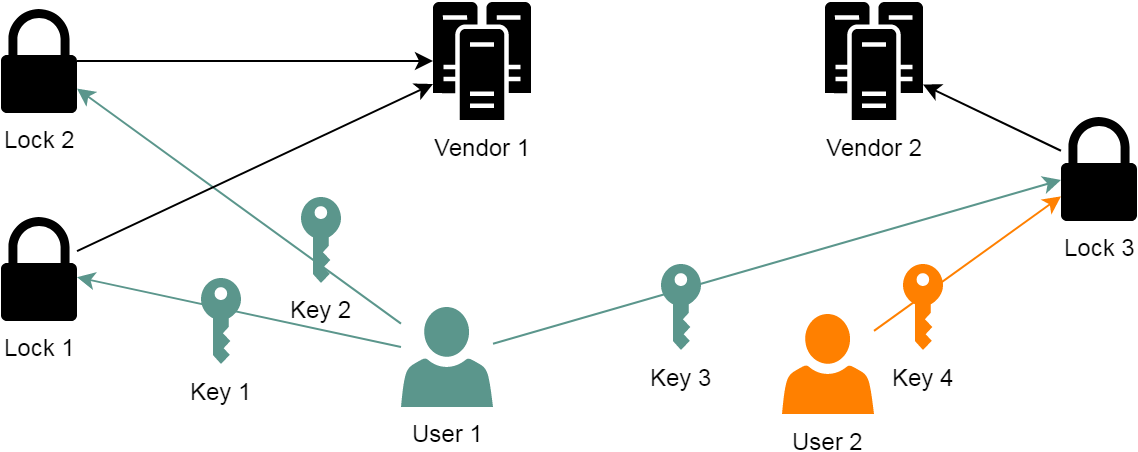
\includegraphics[width=\textwidth]{graphics/pt_network.png}
    		\caption[Beispiel eines von Beziehungen im Prototypen-Netzwerk]{Beispiel von Beziehungen eines Netzwerks, welches aus der Definition des Prototypen entstehen könnte}
    		\label{fig:pt_network}
    	\end{figure}
        \noindent Je nach Teilnehmertyp werden erlaubte Operationen innehalb des Netzwerkes mittels der \gls{acl} eingeschränkt. 
        Die Zugriffskontrolle für den Teilnehmertyp ,,Nutzer`` erfolgt zusätzlich auf einer feingranulareren Ebene über ein dafür angelegtes Attribut \colorbox{light-gray}{\lstinline{UserRole}} mit dem in \fref{tab:prototype_rbac} dargestellten Berechtigungskonzept. 
        Es ist rollenbasiert und ist zu einem großen Teil an \fref{tab:rbac} angelehnt. 
        Anders ist jedoch, dass angelehnt an öffentliche Netzwerke, alle Nutzer des Netzwerkes alle Informationen, die in dieser gespeichert wurden einsehen, aber nicht verändern können. 
        Wie in \fref{tab:prototype_rbac} verdeutlicht, gibt es die Rollen ,,Besitzer`` und ,,Gast`` mit unterschiedlichen Berechtigungen (\ref{fa:3}, \ref{fa:4}). 
        \begin{table}[H]
		    {\footnotesize
		    \centering
            \begin{tabular}{|m{0.14\textwidth}|m{0.14\textwidth}|m{0.14\textwidth}|m{0.14\textwidth}|m{0.14\textwidth}|m{0.14\textwidth}|}
                \hline
                \textbf{Rolle/Recht} &\textbf{Unlock}  & \textbf{Log einsehen}  & \textbf{Nutzer verwalten}  & \textbf{Rollen\-verwal\-tung} & \textbf{Schloss zurück\-setzen}  \\ \hline
                \textbf{Owner}       & \checkmark      & \checkmark             & \checkmark                 & \checkmark                    & \checkmark                       \\ \hline
                \textbf{Guest}       & \checkmark      & \checkmark             & ~                          & ~                             & ~                                \\ \hline
            \end{tabular}
            }
            \caption[Rollenbasierte Zugangskontrolle des Prototypen]{Rollenbasierte Zugangskontrolle des Prototypen. Ist ein Haken gesetzt, so wird der Rolle in der Spalte links das Recht aus der entsprechnenden Spalte gewährt.}
            \label{tab:prototype_rbac}
        \end{table}
        \noindent Die Rolle des Owners wird als Asset modelliert. 
        Ein Nutzer, der ein OwnerAsset besitzt, hat gleichzeitig die Rolle ,,Owner`` inne.
        \noindent Bei Initialisierung des Netzwerkes wird dem Framework gemäß eine Admin-Card erstellt, welche zunächst lediglich dazu dient dem Besitzer auch dessen Rolle zuzuweisen.
        Im Normalfall wird die Admin-Card gar nicht weiter verwendet. \todo[color=cyan]{weiter ausfüren}
        \medskip\\
        \noindent Schlüssel werden als Asset repräsentiert und von Nutzern verwendet, um ein Schloss zu öffnen(\ref{fa:2}). 
        Optional können die Schlüssel mit einem Ablaufzeitpunkt zeitlich eingeschränkt sein(\ref{fa:5}). 
        Es wird ein Schlüssel je Nutzer und Schloss ausgestellt. 
        Somit gäbe es beispielsweise bei zwei Schlössern \colorbox{light-gray}{\lstinline{L1,L2}} und einem Nutzer \colorbox{light-gray}{\lstinline{U1}} im Netzwerk zwei Schlüssel: \colorbox{light-gray}{\lstinline{U1arwL1,U1arwL2}}. \\
        Schlüssel sind nach Erstellung nicht modifizierbar und werden, falls ein Ablaufzeitpunkt angegeben wurde gelöscht. \\
        Beim Öffnen des Schlosses wird das Schlüsselasset mittels einer Funktion ,,Schloss öffnen`` an Schloss gesendet.
        Wird das Schloss wieder verriegelt, so sendet das Schloss das Asset wieder an den Nutzer zurück, der es geöffnet hat. \\
        Hiermit kann einerseits sichergestellt werden, dass das Schloss geschlossen ist, wenn dieses keine Schlüsselassets besitzt, andererseits wird jegliche Nutzung des Schlosses auf der Blockchain dokumentiert. 
        \medskip\\
        \noindent Folgende Informationen werden nach disem Konzept also in der Blockchain gespeichert:
        \begin{itemize}[noitemsep]
            \item Wann von wem welches Schloss geöffnet wurde
            \item Welche Person welche Rolle inne hat und vom diese gewährt wurde
        \end{itemize}
        
    \subsubsection{Implementierungs- und Konfigurationsdetails}
        \paragraph{\textrm{Models}}\hspace{0cm}\smallskip\\
            Participant Types:
            \begin{lstlisting}[caption={Participant Types},label=prototype_pariticipants,captionpos=b]
participant User identified by userId {
    o String userId
    o String firstName
    o String lastName
	o UserRole role
}

participant Vendor identified by vendorServerId {
	o String vendorServerId
	o DateTime lastUpdate
	o Version version
}

participant Lock identified by lockId {
    o String lockId
    o String name
    o DateTime[] unlockLog
	o LockState state
	o Version Version
	--> Vendor vendorId
}
        \end{lstlisting}
            
            \begin{itemize}[noitemsep]
                \item Ein Asset-Typ eines Schlüssels, welcher je Nutzer und Schloss ausgestellt wird
                \item Um \gls{dos} zu vermeiden, etwas ähnliches wie Mutex-Token? z.B. wenn Tür offen ist, dann hat sie genau diesen einen Token
                \item 
            \end{itemize}
            
            Asset Types:
            \begin{lstlisting}[caption={Asset Types},label=prototype_assets,captionpos=b]
asset LockKey identified by keyId {
    o String keyId
    o DateTime expirationDate
    o DateTime[] useLog
    --> Lock lockId
    --> User owner
    --> User issuer
}

asset AdminToken identified by adminId {
	o String adminId
	o DateTime granted
	o DateTime revoked
	o AdminTokenState state
	--> User issuer
    --> User grantee
}
            \end{lstlisting}
        
            Transaction Types:
            \begin{lstlisting}[caption={Relevante Transaktionen},label=prototype_transactions,captionpos=b]
transaction Unlock {
    --> LockKey lockKey
    --> Lock lock
}

transaction GrantUnlock {
    --> LockKey lockKey //Key asset
    --> Lock lock //Lock on which the key can be used
	o DateTime expirationDate optional
    --> User issuer
    --> User grantee
}

transaction RevokeUnlock {
    --> LockKey lockKey //Key asset
    --> Lock lock //Lock on which the key can be used
    --> User issuer
    --> User revokee
}

transaction GrantAdmin {
    --> User issuer
    --> User grantee
}

transaction RevokeAdmin {
    --> User issuer
    --> User revokee
}
            \end{lstlisting}
            
            \begin{itemize}[noitemsep]
                \item Transaktionen bekommen aus dem Systemnamespace schon einen Timestamp und eine ID
                \item OpenDoor
                \item User (AddUser, DeleteUser, ChangeUserRole)
                \item TimeSlot (AddTimeSlot, DeleteTimeSlot, ChangeGuestTimeSlot)
            \end{itemize}
    
    \paragraph{\textrm{Transaction Functions}}
    
    \paragraph{\textrm{Access Control Rules}}\hspace{0cm}\\
        Die Vorgehensweise bei der Definition der \gls{acl}s ist sogenanntes ,,Whitelisting``. 
        Es werden also grundsätzlich alle Operationen auf alle Ressourcen verboten und nur einzelne bestimmte Aktionen von bestimmten Teilnehmern, teilweise nur unter bestimmten Bedinungen erlaubt. 
        Da in Hyperledger Composer die einzelnen Regeln geordnet nacheinander evaluiert werden, müssen zunächst alle erlaubten Aktionen definiert und zum Schluss alle verweigert werden. 
        Eine ausführliche auflistung aller Regeln befindet sich im Anhang\todo[color=orange]{Referenz einfügen}. 
        Beispielsweise:
        \missingfigure{Komplettes Regelwerk für eine Ressource als Beispiel}
        
        Zusammenfassung der implementierten regeln auflisten.
        \begin{itemize}[noitemsep]
            \item 
        \end{itemize}
        
    \paragraph{Query Definitions}
    

    Notizen für den Prototypen:
    \begin{itemize}[noitemsep]
        \item How to ensure a consistent state across all entities?...
        \item keine Anonymisierung, da der Access Log auditable sein muss
        \item Hyperledger bietet CA für Identitäten, Authentifizierung \textrightarrow\ wie ist das bei Composer?
        \item \begin{itemize}
            \item erlaubt Sicherheitseinstellungen beim Erstellen des REST-API-Servers
            \item API Key
            \item Authentication mit Passport
            \item explorer Test interface ?
            \item dynamic logging
            \item event publication over websockets
            \item TLS enable/\-disable
        \end{itemize}
    \end{itemize}
    